%% LaTeX2e class for student theses
%% thesis.tex
%% 
%% Based on SDQ KIT Template by Erik Burger
%%
%% Karlsruhe Institute of Technology
%% Institute for Automation and Applied Informatics
%% AIDA Research Group
%%
%% Nicole Ludwig
%% nicole.ludwig@kit.edu
%%
%% Version 1.3, 20.11.2018

%% Available page modes: oneside, twoside
%% Available languages: english, ngerman
%% Available modes: draft, final
\documentclass[twoside, english]{thesisIAI}

%% ---------------------------------
%% | Additonal Packages |
%% ---------------------------------

\newcommand{\R}{\mathbb{R}}
\renewcommand{\P}{\mathbb{P}}
\newcommand{\set}[1]{\{#1\}}

\usepackage{tikz}
\usetikzlibrary{shapes}
\usetikzlibrary{plotmarks}
\usetikzlibrary{fit}
\usetikzlibrary{overlay-beamer-styles}
\usetikzlibrary{positioning}
\usetikzlibrary{calc}
\usetikzlibrary{decorations.pathreplacing}
\usetikzlibrary{decorations.pathmorphing}
\definecolor{lightblue}{RGB}{189,216,238}

\usepackage{etoolbox}
\newcommand{\R}{\mathbb{R}}

\newcommand{\set}[1]{\{#1\}}
\newcommand{\func}[3]{#1\colon #2 \rightarrow #3}

\DeclareMathOperator{\CRPS}{CRPS}

%% ---------------------------------
%% | Information about the thesis  |
%% ---------------------------------

%% Name of the author
\author{Pavel Zwerschke}

%% Title (and possibly subtitle) of the thesis
\title{Nonparametric Distributional Regression Models for Probabilistic Energy Forecasting}

%% Type of the thesis 
%\thesistype{Master's Thesis}
\thesistype{Bachelor's Thesis}
%\thesistype{Seminar Paper}

%% Change the faculty here
%\faculty{Seminar}
%\faculty{Engineering}
\faculty{Informatics}
%\faculty{Economics}

%% The advisors are PhDs or Postdocs
\advisorone{Advisor One}
%% The second advisor can be omitted
\advisortwo{Advisor Two}

%% Please enter the start end end time of your thesis
\editingtime{Start Date}{End Date}

\settitle

%% Please do not change anything in this tex file without talking to your supervisor
%% LaTeX2e class for student theses
%% format.tex
%% 
%% Based on SDQ KIT Template by Erik Burger
%%
%% Karlsruhe Institute of Technology
%% Institute for Automation and Applied Informatics
%% AIDA Research Group
%%
%% Nicole Ludwig
%% nicole.ludwig@kit.edu
%%
%% Version 1.2.1, 2018-10-11

%% This file switches between the official reviewers and addresses of the faculties 

\ifthenelse{\equal{\thefaculty}{Seminar}}{\uppertitleback}{
	\ifthenelse{\equal{\thefaculty}{Engineering}}{\uppertitleback{Karlsruher Institut für Technologie\\ Fakultät für Maschinenbau\\ Postfach 6980\\ 76128 Karlsruhe}}{
		\ifthenelse{\equal{\thefaculty}{Informatics}}{\uppertitleback{Karlsruher Institut für Technologie\\ Fakultät für Informatik\\ Postfach 6980\\ 76128 Karlsruhe}}{\uppertitleback{Karlsruher Institut für Technologie \\ Fakultät für Wirtschaftswissenschaften \\ Kollegiengebäude am Kronenplatz \\ Geb. 05.20, 3. OG, Raum 3C-05 \\ 76133 Karlsruhe}}}}

\ifthenelse{\equal{\thefaculty}{Informatics}}{\reviewerone{Prof. Dr. Veit Hagenmeyer}}{\reviewerone{apl. Prof. Dr. Ralf Mikut}}

\ifthenelse{\equal{\thefaculty}{Seminar}}{\reviewertwo{}}{
	\ifthenelse{\equal{\thefaculty}{Informatics}}{\reviewertwo{Prof. Dr. Achim Streit}}{
		\ifthenelse{\equal{\thefaculty}{Engineering}}{\reviewertwo{Prof. Dr. Veit Hagenmeyer}}{\reviewertwo{Prof. Dr. Wolf Fichtner}}}}

\ifthenelse{\equal{\thefaculty}{Seminar}}{\facultyname{Energy Informatics Seminar}}{
	\ifthenelse{\equal{\thefaculty}{Engineering}}{\facultyname{\iflanguage{english}{at the Department of Mechanical Engineering}{an der Fakultät für Maschinenbau}}}{
		\ifthenelse{\equal{\thefaculty}{Informatics}}{\facultyname{\iflanguage{english}{at the Department of Informatics}{an der Fakultät für Informatik}}}{
		\facultyname{\iflanguage{english}{at the Department of Economics and Management}{an der Fakultät für Wirtschaftswissenschaften}}}}}
		
		
		




%% --------------------------------
%% | Settings for word separation |
%% --------------------------------

%% Describe separation hints here.
%% For more details, see 
%% http://en.wikibooks.org/wiki/LaTeX/Text_Formatting#Hyphenation
\hyphenation{
% me-ta-mo-del
}

%% --------------------------------
%% | Bibliography                 |
%% --------------------------------

% Please make sure your bibfiles name is thesis.bib and is located in the tex subfolder
\usepackage[                 % !! what about the ``biblatex.cfg''?
        backend=bibtex8,      % (bibtex), bibtex8, biber
%        %
        style=authoryear,		 %numeric-comp,
%        bibstyle=,          % should not be used without citestyle and vice versa
%        citestyle=,
%        natbib=true,
        %
%        sorting=nty,        % (nty), nyt, nyvt, anty, anyt, anyvt, debug, none
%        sortlos=los,        % bib, (los)
%        sortcites=false,    % false
%        maxnames=2,         % <integer> (3)
				maxcitenames=2,      % sets the maximum numbers of authors before abbreviated to et al in text
				maxbibnames=25,       % sets the maximum numbers of authors before abbreviated to et al in bibliography
%        minnames=1,         % (1)
%        maxitems=3,         % (3)
%        minitems=1,         % (1)
%        autocite=,          % inline, footnote, superscript, ...
%        autopunct=true,     % true
%        babel=none,         % (none), hyphen, other, other*
%        block=none,         % (none), space, par, nbpar, ragged
        hyperref=true,      % false
%        backref=false,      % false
%        indexing=false,     % true, (false), cite, bib
%        refsection=none,    % (none), part, chapter, section, subsection
%        refsegment=none,    % (none), part, chapter, section, subsection
%        citereset=none,     % (none), part, chapter, section, subsection
%        abbreviate=true,    % true
%        date=long,          % short, (long)
%        urldate=short,      % (short), long
%        defernums=false,    % false
%        punctfont=false,    % false
        %
%        mincrossrefs=2,     % 2
        bibencoding=inputenc,   % (ascii), inputenc, <encoding>
        %%
%        keywsort=false,     % false
    %
%     useauthor=false,   % true
%     useeditor=false,   % true
%        useprefix=true,     % false
    %
%        pagetracker=true,   % true, (false), page, spread
%     citetracker=true,   % true, (false), context, strict, constrict
%     ibidtracker=true,   % true, (false), context, strict, constrict
%     opcittracker=true,   % true, (false), context, strict, constrict
%     loccittracker=true, % true, (false), context, strict, constrict
%        terseinits=true,    % false
%     labelalpha=true,   % false
%     labelnumber=true,   % false
%     labelyear=true,   % false
%     singletitle=true,   % false
      uniquename=init,   % true, (false), init
%
        doi=false,
        url=false,
				isbn = false,
        giveninits = true % render first/middle names as initals
            ]{biblatex}
	
\makeatletter
\def\blx@maxline{77}
\makeatother
	
	\bibliography{tex/thesis}
   
      %  \DefineBibliographyStrings{ngerman}{%
         %   bibliography     = {Literaturverzeichnis},  % = \bibname
         %   references       = {Literatur},             % = \refname
     %   }
        \defbibnote{alphabetic}{%
            Die Literaturangaben sind alphabetisch nach den Namen
            der Autoren sortiert. Bei mehreren Autoren wird nach
            dem ersten Autor sortiert.\par
            Und mit dem neuen \LPack{biblatex}-Paket funktioniert
            das auch, wie man unschwer erkennen kann.\par\bigskip
        }

% -------------------------------------------------------------------------------------------------
%% declare author names as "last, first".
%% Either for the first author only or for all authors
%\DeclareNameFormat{author}{%
%    \ifthenelse{\value{listcount}=1}
%        {#1%                                            % first author
%            \ifblank{#3}{}{\addcomma\space #3}}
%        {#1%                                            % all the other authors (last, first)
%            \ifblank{#3}{}{\addcomma\space #3}}%
%%        {\ifblank{#3}{}{#3\space}%                      % all the other authors (first last)
%%            #1}%
%    \ifthenelse{\value{listcount}<\value{liststop}}
%        {,\space}
%            {}
%}
%
%%http://projekte.dante.de/DanteFAQ/BiblatexReihenfolgeAutoren
%\DeclareNameFormat{last-first}{%
%  \iffirstinits
%    {\usebibmacro{name:last-first}{#1}{#4}{#5}{#7}}
%    {\usebibmacro{name:last-first}{#1}{#3}{#5}{#7}}%
%  \usebibmacro{name:andothers}}
%\DeclareNameFormat{labelname}{%
%   \ifuseprefix
%     {\usebibmacro{name:last-first}{#1}{#4}{#5}{#8}}
%     {\usebibmacro{name:last-first}{#1}{#4}{#6}{#8}}%
%   \usebibmacro{name:andothers}}

%  \DefineBibliographyStrings{english}{%
%    typeeditor = {{}{}},
%    typeeditors = {{}{}},
%    in = {{}{}},
%    inseries = {{}{}},
%    byeditor = {{}{}}
%  }

%-------------------------------------------------------------------------------------------------

%% http://www.golatex.de/biblatex-anpassen-die-x-te-frage-t4657.html
\renewbibmacro*{journal+issuetitle}{%
  \usebibmacro{journal}%
  \setunit*{\addcomma\space}%
  \iffieldundef{series}
    {}
    {\newunit
     \printfield{series}%
     \setunit{\addcomma\space}}%
  \printfield{volume}%
  \setunit*{\addcomma\space}%
  \printfield{number}%
  \setunit{\addcomma\space}%
  \printfield{eid}%
  \setunit{\addspace}%
  \usebibmacro{issue+date}%
  \setunit{\addcolon\space}%
  \usebibmacro{issue}%
  \newunit}

\DeclareFieldFormat[article]{volume}{\bibstring{jourvol}~#1}
\DeclareFieldFormat[article]{number}{\bibstring{number}~#1} 
%\DeclareFieldFormat[article]{edition}{\bibstring{edition}~#1} 

%% http://mrunix.de/forums/showthread.php?t=67386
\DefineBibliographyStrings{english}{jourvol={Vol\adddot}} 
\DefineBibliographyStrings{english}{number={No\adddot}} 
\DefineBibliographyStrings{english}{edition={Ed\adddot}} 

\AtBeginBibliography{%
  % Setzt die Autoren-Vornamen auf Kapitälchen 
  \renewcommand*{\mkbibnamefirst}{\textsc}
  \renewcommand*{\mkbibnamelast}{\textsc}
  \renewcommand*{\mkbibnameprefix}{\textsc}
  \renewcommand*{\mkbibnameaffix}{\textsc}
  
  %%Doppelpunkt nach Namen, kein Punkt
  %\renewcommand*{\labelnamepunct}{\addcolon\space} 
  
  \DeclareFieldFormat{name}{\textsc{#1\isdot}}
  \DeclareFieldFormat{title}{\mkbibemph{#1\isdot}}
  
  %%\DeclareFieldFormat[article]{title}{#1}
  %%\DeclareFieldFormat[article]{title}{\mkbibquote{#1}}
  \renewcommand*{\mkbibquote}[1]{\mkbibemph{#1\isdot}}
 
  % http://tex.stackexchange.com/ ...
  % questions/16716/spell-out-volume-and-edition-in-words-biblatex-in-german
  %\renewcommand*{\mkbibordedition}[1]{\Ordinalstringnum{#1}[f]}
  \renewcommand*{\mkbibordedition}[1]{\ordinalnum{#1}}
} 
\usepackage[toc]{glossaries}

%\glstoctrue

\newacronym{emos}{EMOS}{Ensemble Model Output Statistics}
\newacronym{ecmwf}{ECMWF}{European Centre for Medium-Range Weather Forecasts}
\newacronym{eps}{EPS}{Ensemble Prediction System}
\newacronym{ecc}{ECC}{Ensemble Copula Coupling}
\newacronym{pdf}{PDF}{Probability Distribution Function}
\newacronym{nwp}{NWP}{Numerical Weather Prediction}
\newacronym{crps}{CRPS}{Continuous Ranked Probability Score}
\newacronym{mape}{MAPE}{Mean Absolute Percentage Error}
\newacronym{rmse}{RMSE}{Root Mean Squared Error}


%\renewcommand{\glsnamefont}[1]{\emph{#1}}
\setlength{\glsdescwidth}{0.9\linewidth}

\makeglossaries

%% ====================================
%% ====================================
%% ||                                ||
%% || Beginning of the main document ||
%% ||                                ||
%% ====================================
%% ====================================

%% Set PDF metadata
\setpdf

\begin{document}

\hypersetup{pageanchor=false}

%% Set the title
\maketitle

%% The Preamble begins here
\frontmatter

%% LaTeX2e class for student theses: Declaration of independent work
%% sections/declaration.tex
%% 
%% Karlsruhe Institute of Technology
%% Institute for Program Structures and Data Organization
%% Chair for Software Design and Quality (SDQ)
%%
%% Dr.-Ing. Erik Burger
%% burger@kit.edu
%%
%% Version 1.3.2, 2017-08-01

\thispagestyle{empty}
\null\vfill
\noindent\hbox to \textwidth{\hrulefill} 
\iflanguage{english}{I declare that I have developed and written the enclosed
\ifthenelse{\equal{\thefaculty}{Engineering}}{thesis}{\ifthenelse{\equal{\thefaculty}{Informatics}}{thesis}{paper}} completely by myself, and have not used sources or means without
declaration in the text.}%
{Ich versichere wahrheitsgemäß, die Arbeit
selbstständig angefertigt, alle benutzten Hilfsmittel vollständig und genau
angegeben und alles kenntlich gemacht zu haben, was aus Arbeiten anderer
unverändert oder mit Änderungen entnommen wurde.}
 
 
%% ---------------------------------------------
%% | Replace PLACE and DATE with actual values |
%% ---------------------------------------------
\textbf{PLACE, DATE}
\vspace{1.5cm}
 
\dotfill\hspace*{8.0cm}\\
\hspace*{2cm}(\theauthor) 
\cleardoublepage

\setcounter{page}{1}
\pagenumbering{roman}

%% ----------------
%% |   Abstract   |
%% ----------------
 
%% For theses written in English, an abstract both in English
%% and German is mandatory.
%%
%% Seminar Papers written in English need only an English abstract.
%%
%% For theses written in German, a German abstract is sufficient.
%%
%% The text is included from the following files:
%% - sections/abstract
%% - sections/zusammenfassung

\pdfbookmark[1]{Abstract}{Abstract}

\chapter*{Abstract}

\begin{center}
  \begin{minipage}{12cm}
    \begin{sloppypar}
      As the share of electricity from regenerative sources is growing constantly, 
      it makes sense to predict the power generation of these sources. 
      In order to model the uncertainty of a forecast, one often predicts the probability 
      distribution of the corresponding random variable. There are many different nonparametric machine learning approaches 
      to the solar power generation forecasting problem. Hence, this thesis compares three approaches 
      in order to predict solar power generation, namely Quantile Random Forests, Nearest Neighbor Quantile Filters and 
      Spline Quantile Functions RNN. The performance of the models is evaluated on the Global Energy Forecasting Competition 2014 
      dataset. 
      We see that the Quantile Regression Forests manage to get the best score of \(0.01873\) following 
      the Nestest Neighbor Quantile Filters model with a score of \(0.0194\) and the Spline Quantile Functions RNN model with a score of \(0.02041\). 
    \end{sloppypar}
  \end{minipage}
\end{center}

\hypersetup{pageanchor=true}
%% ------------------------
%% |   Table of Contents  |
%% ------------------------
\tableofcontents
\listoffigures
\listoftables

\printglossary[title=Abbreviations, toctitle=List of Abbreviations, 
style=super, nogroupskip, nopostdot, nonumberlist]

%% -----------------
%% |   Main part   |
%% -----------------

\mainmatter

\chapter{Introduction}
\label{ch:Introduction}

\stress{\textbf{Disclaimer to this document:} 
This is a template with some additional thesis information and a sample structure. 
The structure includes the chapters most commonly needed in a thesis. 
Neither the order nor the chapter titles are fixed and will most likely 
have to be adapted to your specific thesis. 
However, the notes here should help you to get an idea what each chapter 
could be about and how to use this template. 
When in doubt, please talk to your supervisor(s).}

Your thesis should start with an introduction. The introduction is supposed to motivate your thesis.
Discuss the relevance of your topic, why are you looking into it, why is it relevant in the field? Cite important research related to your motivation.
Briefly state the problem as in the abstract and repeat the contribution, for example in the form of research questions. 

Give an outline of your thesis.

Testing the glossaries package \gls{rmse}


Below, you will find an example figure (\Cref{fig:example}). Please use the caption of your figures to describe everything in the figure, additionally to what you have written about the figure in the text. Everyone should be able to understand the figure just reading its caption.

\begin{figure}[h!]%
\centering
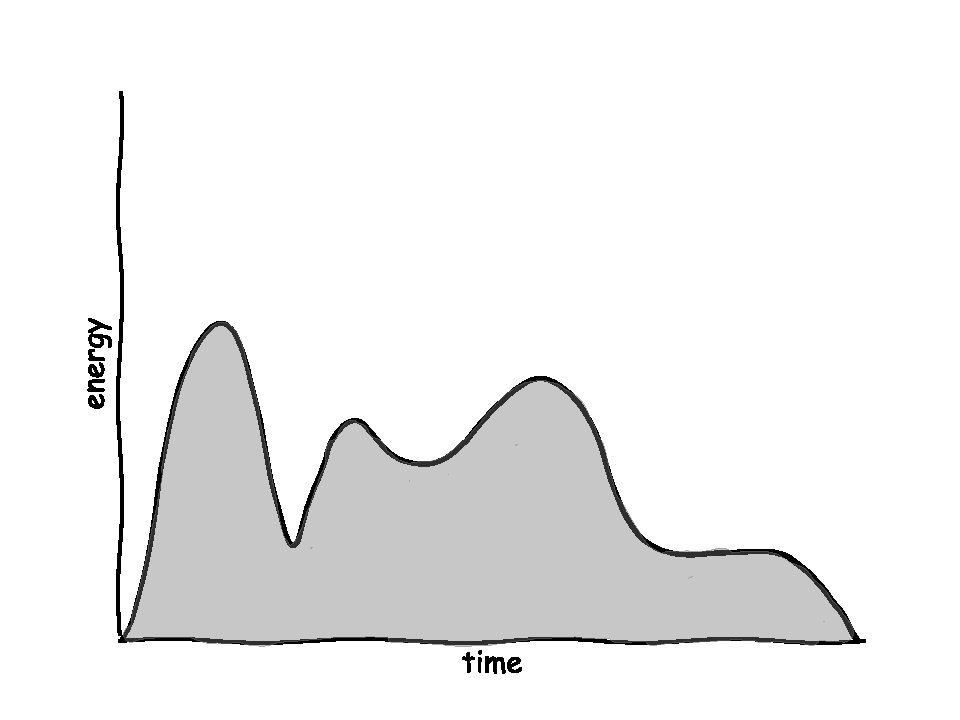
\includegraphics[width=0.5\columnwidth]{plots/Figure_2_demand}%
\caption{This is an example figure. It shows a fictional demand of energy (in grey) over time.}%
\label{fig:example}%
\end{figure}

\section{The GEFCom2014 Dataset}
\label{sec:gefcom-dataset}

In order to compare different energy forecasting methods, 
\Textcite{Hong2016} organized the Global Energy Forecasting Competition 2014 (GEFCom2014), 
a probabilistic energy forecasting competition with four tracks: 
electric load, electric price, wind power and solar power forecasting. 
The competition attracted 581 participants from 61 countries. 

The Global Energy Forecasting Competition took place the first time in 2012. 
In the 2014 competition, they upgraded the competition with three features: 
\begin{enumerate}
    \item instead of point forecasts, probabilistic forecasts were used;
    \item four forecasting tracks were used: electric load (L track), 
    electric price (P track), wind power (W track) and solar power (S track);
    \item incremental data releases on a weekly basis to mimic real world forecasting.
\end{enumerate}

In this thesis, we will only look at the solar power track. 
In this track, the task is to predict the power generation of three 
solar power plants (the so called zones) in Australia. 
The prediction is on a rolling basis for \(\SI{24}{\hour}\) ahead. 
The forecasts are to be issued at midnight each day for the next \(24\) hours. 
\(15\) tasks are provided for the challenge. In each one, the participants need to 
provide one month of forecasts, so \(28\)-\(31\) days.
For the forecasts, different prediction variables from the 
European Centre for Medium-Range Weather Forecasts (ECMWF) are provided. 
They are shown in Table \ref{table:predictors}.
Power measurements are also provided, but only over the training period. 

In order to become familiar with the data, only the last twelve of the 15 available tasks 
from April 2013 to June 2014 counted towards the final score.
The final score was calculated using a linear increasing weighted mean over the scores from the different tasks: 
The first task got weight \(1/78\), the second \(2/78\), etc. 
in order to promote models that improve over time. The division by \(78\) is so that the 
weights sum to \(1\).
Since we will evaluate the models on the dataset as a whole instead of on a monthly different basis, 
we will take the mean over the \(12\) different losses.

\begin{table}[ht]
\caption[Predictors for the GEFCom2014-S track]{Predictors for the GEFCom2014-S track \par Adapted from Table 10 in \cite{Hong2016}}
\label{table:predictors}
\rowcolors{2}{white}{gray!25}
\footnotesize
\begin{tabularx}{\textwidth}{llX}
    \toprule
    \tableheads Variable name & \tableheads Units & \tableheads Comments \\
    \midrule
    Total column liquid water (tclw) & \(\si{\kilo\gram\per\square\metre}\) & Vertical integral of cloud liquid water content \\
    Total column ice water (tciw) & \(\si{\kilo\gram\per\square\metre}\) & Vertical integral of cloud ice water content \\
    Surface pressure (SP) & \(\si{\pascal}\) & \\
    Relative humidity at \(\SI{1000}{\milli\barsi}\) (r) & \(\%\) & Relative humidity is defined with respect to saturation of
                                                                  the mixed phase, i.e., with respect to saturation over ice
                                                                  below \(\SI{-23}{\degreeCelsius}\) and with respect to saturation over water 
                                                                  above \(\SI{0}{\degreeCelsius}\). In the regime in between, a quadratic
                                                                  interpolation is applied. \\
    Total cloud cover (TCC) & \(0\)-\(1\) & TCC derived from model levels using the
                                            model's overlap assumption \\
    \(10\)-metre \(U\) wind component (\(10u\)) & \(\si{\metre\per\second}\) & \\
    \(10\)-metre \(V\) wind component (\(10v\)) & \(\si{\metre\per\second}\) & \\
    \(2\)-metre temperature (\(2T\)) & \(\si{\kelvin}\) & \\
    Surface solar rad down (SSRD) & \(\si{\joule\per\square\metre}\) & Accumulated field \\
    Surface thermal rad down (STRD) & \(\si{\joule\per\square\metre}\) & Accumulated field \\
    Top net solar rad (TSR) & \(\si{\joule\per\square\metre}\) & Net solar radiation at the top of the atmosphere. Accumulated field \\
    Total precipitation (TP) & \(\si{\metre}\) & Convective precipitation \(+\) stratiform precipitation (CP + LSP). Accumulated field \\
    \bottomrule
\end{tabularx}
\end{table}
\chapter{Related Work}
\label{ch:RW}

This chapter is supposed to summarise previous work of other researchers related to your topic.
The aim is to give an overview of existing literature while highlighting differences and similarities to this thesis.

There are several forms of citations you can use throughout your thesis. For example

\begin{itemize}
	\item Direct citation of results, an approach or similar
	\item[] \Textcite{Fan.2015} find that their method improves the benchmark.
	\item Indirect citation
	\item[] Recent research highlights the importance of this method \Parencite{Fan.2015}.
	\item Direct citation
	\item[] \textquote{\emph{Energy optimisation in buildings is important}} \Parencite{Fan.2015}.
\end{itemize}


Please choose a coherent citation style throughout the thesis.

\chapter{Methodology/ Foundations}
\label{ch:methods}

This chapter should introduce to the theoretical background of your thesis. Any method abd concept you use to obtain the results, should be introduced and explained. Additionally, you should describe how you evaluate/ solve/ approach the research question which you are answering in your thesis. Depending on your thesis topic and structure, foundations and methodology can both be part of one chapter, or separated into two different chapters. If you are unsure what to do, or what the differences are, please contact your supervisor.

\section{Method 1}

This is an example for a simple equation without equation numbering.
$$
\sum\limits_{i=1}^{n}{x_i}
$$

You can also use equation numbering if you need to refer to an equation later \eg \Cref{eq:ex1}.


\begin{equation}
a^2 + b^2 = c^2
\label{eq:ex1}
\end{equation}

Additionally, simple equations can be put inline with the text, for example, $x \in X$. Remember to set all variables in math font \ie all $x$, $i$ and so on.

\section{Method 2}

\dots


\chapter{Evaluation}
\label{ch:Evaluation}

In this chapter, we will look at the results of the different models. 
We first evaluate which features are most important for the models using 
permutation feature importance, then we will look at the pinball scores from 
that are used in the competition. Finally, we will look at how the models performed 
considering another scoring function, the Energy score.

\section{Feature importance}
\label{sec:feature-importance}

One way to determine the importance of a feature for a model is called 
permutation feature importance. Here, the model is trained like usual but for the prediction 
step, we don't use the normal test data, but a modified dataset where one feature is 
shuffled. Like that, the model cannot use the information of this feature properly 
and will most likely perform worse. The performance on the shuffled dataset is 
then divided by the performance on the regular test set. A value close to \(1\) 
indicates that the feature is not that important because the model doesn't perform 
much worse than before. The higher the quotient, the more important the feature is for the model.
Since our time series heavily depends of the time of day, it makes sense 
not to shuffle the whole feature but only the equivalence classes of each hour, 
i.e. the values at \(1\) AM are shuffled, the values at \(2\) AM are shuffled, etc.

Figure \ref{fig:feature-importance} 
shows the results of the permutation feature importance calculation.

\begin{figure}[h!]
    \section{Feature importance}
\label{sec:feature-importance}

One way to determine the importance of a feature for a model is called 
permutation feature importance. Here, the model is trained like usual but for the prediction 
step, we don't use the normal test data, but a modified dataset where one feature is 
shuffled. Like that, the model cannot use the information of this feature properly 
and will most likely perform worse. The performance on the shuffled dataset is 
then divided by the performance on the regular test set. A value close to \(1\) 
indicates that the feature is not that important because the model doesn't perform 
much worse than before. The higher the quotient, the more important the feature is for the model.
Since our time series heavily depends of the time of day, it makes sense 
not to shuffle the whole feature but only the equivalence classes of each hour, 
i.e. the values at \(1\) AM are shuffled, the values at \(2\) AM are shuffled, etc.

Figure \ref{fig:feature-importance} 
shows the results of the permutation feature importance calculation.

\begin{figure}[h!]
    \input{plots/feature_importance}
    \caption[Feature importance]{Feature importance. 
    The table shows the permutation feature importance quotients. 
    The permutation feature importance quotient is 
    the performance of the model with shuffled feature 
    divided by the performance of the model without shuffled features. 
    A higher value indicates a more important feature.}
    \label{fig:feature-importance}
\end{figure}
    \caption[Feature importance]{Feature importance. 
    The table shows the permutation feature importance quotients. 
    The permutation feature importance quotient is 
    the performance of the model with shuffled feature 
    divided by the performance of the model without shuffled features. 
    A higher value indicates a more important feature.}
    \label{fig:feature-importance}
\end{figure}

\section{Pinball Loss}
\label{sec:elaboration-pinball-loss}

As stated in section \ref{sec:pinball-loss-explanation}, the pinball loss is 
used to determine the performance of the different models. 
It is calculated by taking the average over all pinball losses for each time 
point and zone in the dataset. 

Table \ref{table:pinball-loss} and Figure \ref{fig:pinball-loss} show the 
losses of the models for task 4 to task 15 (July 2013 to June 2014). 
We can see that the QRF and NNQF model perform similarly and that the 
SQF-RNN model performs better than the other two during the months from October to Febuary.
Another thing to note is that the DeepAR model always performs worse than the SQF-RNN model.

\begin{table}[ht]%
    \footnotesize
    \hspace*{25pt} % make kind of centering
    \begin{minipage}{\textwidth}
    \renewcommand{\b}[1]{\textbf{#1}}
    \rowcolors{2}{white}{gray!25}
    \begin{tabular}{c|cccccc}
        \toprule \noalign{\smallskip}
        Task & \(4\) & \(5\) & \(6\) & \(7\) & \(8\) & \(9\) \\
        \midrule
        QRF     & \(\b{0.01462}\) & \(\b{0.02022}\) & \(\b{0.01884}\) & \(0.02250\)     & \(0.02258\)     & \(0.02212\)     \\
        NNQF    & \(0.01559\)     & \(0.02091\)     & \(0.01896\)     & \(0.02267\)     & \(0.02330\)     & \(0.02334\)     \\
        SQF-RNN & \(0.02581\)     & \(0.03041\)     & \(0.02451\)     & \(\b{0.01895}\) & \(\b{0.01707}\) & \(\b{0.01833}\) \\
        DeepAR  & \(0.02634\)     & \(0.03649\)     & \(0.02744\)     & \(0.01958\)     & \(0.02579\)     & \(0.02290\)     \\
        \bottomrule
    \end{tabular}
    \vspace*{1em} \\
    \rowcolors{2}{white}{gray!25}
    \begin{tabular}{c|cccccc|c}
        \toprule \noalign{\smallskip}
        Task & \(10\) & \(11\) & \(12\) & \(13\) & \(14\) & \(15\) & Mean \\
        \midrule
        QRF     & \(0.02232\)     & \(\b{0.02012}\) & \(\b{0.01824}\) & \(\b{0.01561}\) & \(\b{0.01355}\) & \(\b{0.01402}\) & \(\b{0.01873}\) \\
        NNQF    & \(0.02333\)     & \(0.02038\)     & \(0.01912\)     & \(0.01673\)     & \(0.01363\)     & \(0.01480\)     & \(0.01940\)     \\
        SQF-RNN & \(\b{0.02002}\) & \(0.02104\)     & \(0.02204\)     & \(0.01684\)     & \(0.01338\)     & \(0.01648\)     & \(0.02041\)     \\
        DeepAR  & \(0.02320\)     & \(0.02612\)     & \(0.02424\)     & \(0.02282\)     & \(0.01865\)     & \(0.01889\)     & \(0.02437\)     \\
        \bottomrule
    \end{tabular}
    \end{minipage}

    \caption[Pinball loss]{Pinball loss. 
    Each task is one month in the training period. 
    Task 4 represents July 2013, Task 5 August 2013, etc. up until June 2014.
    The pinball loss is calculated by averaging 
    over all pinball losses for each time point and zone.}
    \label{table:pinball-loss}
\end{table}

\begin{figure}[ht]
    \centering
    \section{Pinball Loss}
\label{sec:elaboration-pinball-loss}

As stated in section \ref{sec:pinball-loss-explanation}, the pinball loss is 
used to determine the performance of the different models. 
It is calculated by taking the average over all pinball losses for each time 
point and zone in the dataset. 

Table \ref{table:pinball-loss} and Figure \ref{fig:pinball-loss} show the 
losses of the models for task 4 to task 15 (July 2013 to June 2014). 
We can see that the QRF and NNQF model perform similarly and that the 
SQF-RNN model performs better than the other two during the months from October to Febuary.
Another thing to note is that the DeepAR model always performs worse than the SQF-RNN model.

\begin{table}[ht]%
    \footnotesize
    \hspace*{25pt} % make kind of centering
    \begin{minipage}{\textwidth}
    \renewcommand{\b}[1]{\textbf{#1}}
    \rowcolors{2}{white}{gray!25}
    \begin{tabular}{c|cccccc}
        \toprule \noalign{\smallskip}
        Task & \(4\) & \(5\) & \(6\) & \(7\) & \(8\) & \(9\) \\
        \midrule
        QRF     & \(\b{0.01462}\) & \(\b{0.02022}\) & \(\b{0.01884}\) & \(0.02250\)     & \(0.02258\)     & \(0.02212\)     \\
        NNQF    & \(0.01559\)     & \(0.02091\)     & \(0.01896\)     & \(0.02267\)     & \(0.02330\)     & \(0.02334\)     \\
        SQF-RNN & \(0.02581\)     & \(0.03041\)     & \(0.02451\)     & \(\b{0.01895}\) & \(\b{0.01707}\) & \(\b{0.01833}\) \\
        DeepAR  & \(0.02634\)     & \(0.03649\)     & \(0.02744\)     & \(0.01958\)     & \(0.02579\)     & \(0.02290\)     \\
        \bottomrule
    \end{tabular}
    \vspace*{1em} \\
    \rowcolors{2}{white}{gray!25}
    \begin{tabular}{c|cccccc|c}
        \toprule \noalign{\smallskip}
        Task & \(10\) & \(11\) & \(12\) & \(13\) & \(14\) & \(15\) & Mean \\
        \midrule
        QRF     & \(0.02232\)     & \(\b{0.02012}\) & \(\b{0.01824}\) & \(\b{0.01561}\) & \(\b{0.01355}\) & \(\b{0.01402}\) & \(\b{0.01873}\) \\
        NNQF    & \(0.02333\)     & \(0.02038\)     & \(0.01912\)     & \(0.01673\)     & \(0.01363\)     & \(0.01480\)     & \(0.01940\)     \\
        SQF-RNN & \(\b{0.02002}\) & \(0.02104\)     & \(0.02204\)     & \(0.01684\)     & \(0.01338\)     & \(0.01648\)     & \(0.02041\)     \\
        DeepAR  & \(0.02320\)     & \(0.02612\)     & \(0.02424\)     & \(0.02282\)     & \(0.01865\)     & \(0.01889\)     & \(0.02437\)     \\
        \bottomrule
    \end{tabular}
    \end{minipage}

    \caption[Pinball loss]{Pinball loss. 
    Each task is one month in the training period. 
    Task 4 represents July 2013, Task 5 August 2013, etc. up until June 2014.
    The pinball loss is calculated by averaging 
    over all pinball losses for each time point and zone.}
    \label{table:pinball-loss}
\end{table}

\begin{figure}[ht]
    \centering
    \input{plots/pinball_loss}
    \caption[Pinball loss]{Pinball loss. 
    This graph plots the losses of the models for each month of the dataset competition.}
    \label{fig:pinball-loss}
\end{figure}

As described in section \ref{sec:implementation-nnqf}, 
we only use one neural network with more hidden nodes instead of 
separate neural networks for each node. 
The pinball loss for training the model with \(99\) different neural networks 
is \(0.01998\), so the version with one neural network performs approximately the 
same while being noticably faster. 
Another modification to the original algorithm proposed by \Textcite{Ordiano2019} 
is sorting the predicted quantiles instead of taking the maximum as described in 
section \ref{sec:implementation-nnqf}. The avergae pinball loss over all tasks for the second is 
\(0.02742\), so sorting the quantiles instead of taking the maximum of the previous quantile 
results in a noticable performance improvement.
    \caption[Pinball loss]{Pinball loss. 
    This graph plots the losses of the models for each month of the dataset competition.}
    \label{fig:pinball-loss}
\end{figure}

As described in section \ref{sec:implementation-nnqf}, 
we only use one neural network with more hidden nodes instead of 
separate neural networks for each node. 
The pinball loss for training the model with \(99\) different neural networks 
is \(0.01998\), so the version with one neural network performs approximately the 
same while being noticably faster. 
Another modification to the original algorithm proposed by \Textcite{Ordiano2019} 
is sorting the predicted quantiles instead of taking the maximum as described in 
section \ref{sec:implementation-nnqf}. The avergae pinball loss over all tasks for the second is 
\(0.02742\), so sorting the quantiles instead of taking the maximum of the previous quantile 
results in a noticable performance improvement.
\section{Discussion}
\label{sec:discussion}

In this section, we discuss the results, compare the different 
models and look at potential weaknesses of the competition. 

Looking at Figure \ref{fig:pinball-loss}, we see that NNQF and QRF perform very similarly. 
In the months from October to Febuary, i.e., the summer months since 
Australia is located in the southern hemisphere, we can see that 
the SQF-RNN model performs noticably better than the NNQF and QRF models. 
One explanation could be that the NNQF and QRF models only focus on solar 
radiation but not on total cloud cover.  
In the summer months, the solar energy is influenced in a large part by 
how many clouds are in the sky. Figure \ref{fig:feature-importance} shows us that 
the SQF-RNN model focuses more on total cloud cover. Therefore, 
it performs better in these months. 

When comparing the SQF-RNN and the DeepAR model with 
the Student's \(t\)-distribution in Figure \ref{fig:pinball-loss} and 
Figure \ref{fig:energy-score}, we can see that the DeepAR model 
always performs worse than the SQF-RNN model. 
The nonparametric approach is better than assuming 
that the target variable follows an arbitrary distribution. 
Thus we can conclude that the Student's \(t\)-distribution is not the optimal fit 
and spline quantile functions model the distribution better. 

When looking at the energy score in Figure \ref{fig:energy-score}, 
we can see that the SQF-RNN model outperforms the NNQF model as well as QRF.
One reason why the SQF-RNN works better here is that it takes 
the time series attributes into account because of its RNN structure. 
The NNQF model only uses lag features while the QRF model does not incorporate 
the previous values at all, it only looks at the current time point.

As discussed in Chapter \ref{ch:evaluation}, 
the QRF predictions are capped 
at the top (Figure \ref{fig:predictions-qrf}). 
This is because of the QRF's predictive nature: it generates 
the prediction directly from the previous target data 
and thus cannot predict values 
that are higher than the maximal values of the training set. 
The other two models do not suffer from this because they use 
neural networks to predict the target distribution.

The PIT histograms indicate whether if the forecasting method is probabilistically 
calibrated or if it is over- or underdispersed. If the forecast is not neutrally dispersed, 
it cannot be probabilistically calibrated.
Figure \ref{fig:pit} indicates that the QRF and NNQF model are 
probabilistically calibrated while the PIT histograms of SQF-RNN 
and DeepAR model are skewed and thus their predictive distribution is 
biased in their location.

When we look at the PIT histograms by each hour 
for quantile regression forests in Figure \ref{fig:pit-qrf-by-hour} 
we can observe that the predictions for the night are underdispersed. 
Since the solar plants do not produce energy during the night 
it makes sense to just predict \(0\) for the target variable when there is 
no sunshine.

The NNQF model also suffers a bit from this problem. We can see 
in Figure \ref{fig:pit-nnqf-by-hour} in the time frame 22:00-00:00 that 
there is a high density at \(0\) indicating that the forecast 
was often too high. This can be fixed like in the proposition above.

The hourly PIT histograms for the SQF-RNN and DeepAR model in 
Figure \ref{fig:pit-deepar-by-hour} and Figure \ref{fig:pit-sqf-rnn-by-hour} 
both indicate the same as mentioned above: both predictions are biased 
in their location. One solution would be postprocessing by shifting the 
predictions so that the PITs are approximately symmetric. 

The competition aims to mimic real time solar energy forecasting with 
a \(\SI{24}{\hour}\) forecast horizon. In this scenario, the energy data of 
the previous days would be available. Since the competition organizers want to 
prevent overfitting the data and minimize organizational overhead, 
the target variables are not available for 
the entire month. Since the SQF-RNN model uses the previous time points for the prediction, 
this might be one reason why it does not perform as expected. 
It is the most complicated of the three but has the worst results 
despite taking temporal dependencies into account. 
In order to compare the model fairly with the other competitors, 
we implemented it under competition conditions. A more realistic approach would be 
providing the model with the target data and evaluating it this way.
\section{Conclusion}
\label{sec:conclusion}

In this thesis, we look at three different approaches to probabilistic forecasting 
for solar energy generation and compare them on the GEFCom2014 dataset. 
Results show that the QRF and the NNQF model perform similar without 
hyperparameter optimization and that the QRF model improves after the hyperparameter 
optimization. The SQF-RNN model performs better during the summer months than the other two models. 

The QRF and NNQF model are both underdispersed during the night. This can be dealt with by simply forecasting \(0\). 
Nonparametric models are not always the easiest solution. Sometimes it makes sense to just predict the obvious 
instead of training a complex model.

The discrepancy between the results of the SQF-RNN model and the DeepAR model show us that 
nonparametric models perform better than parametric ones in a context where we don't know the actual probability distribution. 
The pinball loss crowned the QRF model the winner while the energy score marked the SQF-RNN model as winner. 
Different scoring functions emphasize different properties of a forecast -- just because one forecast has a 
better score than another forecast doesn't mean that it is better than the other in every aspect.

Another point to note is that different models perform differently due to different features being 
prioritized: the QRF and NNQF model both prioritize approximately the same features and therefore 
yield similar results. The SQF-RNN model prioritizes other features and performs in some months better 
and in other months worse than the other two models. A model's performance is highly dependent on the input features.
Therefore, it is important to investigate feature selection in detail and to look which explaining features promise the best results. 
Future work could investigate feature selection and preprocessing in more detail. 

As discussed in section \ref{sec:discussion}, the SQF-RNN model does not perform as well as expected 
because the competition does not allow the previous time data to be used as an input value. 
Future work could examine how well the SQF-RNN and DeepAR model perform after fixing this issue, 
i.e., enabling \(\SI{24}{\hour}\) ahead forecasts with previous target data. 

%% --------------------
%% |   Bibliography   |
%% --------------------

%% Add entry to the table of contents for the bibliography
\printbibliography[heading=bibintoc]

%% ----------------
%% |   Appendix   |
%% ----------------
\appendix
%% LaTeX2e class for student theses
%% appendix
%% 
%% Based on SDQ KIT Template by Erik Burger
%%
%% Karlsruhe Institute of Technology
%% Institute for Automation and Applied Informatics
%% AIDA Research Group
%%
%% Nicole Ludwig
%% nicole.ludwig@kit.edu
%%
%% Version 1.2, 2018-10-11


\iflanguage{english}
{\chapter{Appendix}}    % english style
{\chapter{Anhang}}      % german style
\label{ch:appendix}

\section{Proper scoring rules}
\label{sec:proper-scoring-rules}

To measure the error of a probabilistic forecast, one usually uses a 
proper scoring rule. 
Let \(\mathcal{P}\) be a convex class of probability measures on the 
measurable space \((\Omega, \mathcal{A})\).
A \textit{scoring rule} is any extended real-valued function 
\[ \func{S}{\mathcal{P} \times \Omega}{\overline{\R}} \]
such that \(S(P, \cdot)\) is \(\mathcal{P}\)-quasiintegrable for all 
\(P\in \mathcal{P}\).
A scoring rule \(S\) is \textit{proper} relative to a convex subclass 
\(\mathcal{P}_0 \subseteq \mathcal{P}\) if
\[ \int_\Omega S(Q, \omega) \mathrm{d}Q(\omega) \leq \int_\Omega S(P, \omega) \mathrm{d}Q(\omega) \]
for all \(P, Q \in \mathcal{P}_0\). It is \textit{strictly proper} 
if equality holds iff. \(P = Q\).

This property encourages honest and careful quotes by the forecaster. 

\section{CRPS}
\label{ch:crps}

\renewcommand{\d}{\mathrm{d}}

The \gls{crps} is one of the most common 
scoring rules. It is defined as follows: 

\[ \CRPS(F, y) = \int_{-\infty}^\infty \left( F(y) - \mathds{1} \{y \leq x\} \right)^2 \d x, \]
where \(F\) is the CDF of the probabilistic forecast.
We can show that the CRPS can also be written as 
\[ \CRPS(F, y) = 2 \int_0^1 L_\alpha(F^{-1}(\alpha), y) \d \alpha, \]
where \(L_\alpha\) is the pinball loss.
\begin{proof}
    The CRPS can be written as the integral over elementary scoring functions for quantile forecasts: 
    \[ \CRPS(F, y) = 2 \int_0^1 \int_{-\infty}^\infty \mathrm{s}_{\alpha, \eta}(F^{-1}(\alpha), y) \d \eta \d \alpha, \]
    where 
    \[ \mathrm{s}_{\alpha, \eta}(q, y) = \begin{cases}
        1-\alpha, &y\leq \eta < q, \\
        \alpha, &q\leq \eta < y \\
        0, &\text{otherwise}.
    \end{cases} \]

    Let \(\eta < y\). 
    \[ 2 \int_0^1 \mathrm{s}_{\alpha, \eta}(F^{-1}(\alpha), y) \d\alpha = 2 \int_0^{F(\eta)} \alpha \d \alpha = F(\eta)^2 = (F(\eta) - \mathds{1}_{\set{y \leq \eta}})^2. \]
    Let \(\eta \geq y\).
    \[ 2 \int_0^1 \mathrm{s}_{\alpha, \eta}(F^{-1}(\alpha), y) \d\alpha = 2 \int_{F(\eta)}^1 (1-\alpha) \d\alpha = \left[ - (1-\alpha)^2 \right]_{F(\eta)}^1 = (F(\eta) - \mathds{1}_{\set{y \leq \eta}})^2. \]
    Therefore, we get 
    \begin{align*}
        \CRPS(F, y) &= \int_{-\infty}^\infty (F(\eta) - \mathds{1}_{\set{y\leq x}})^2 \d \eta \\
        &= \int_{-\infty}^\infty 2 \int_0^1 \mathrm{s}_{\alpha, \eta}(F^{-1}(\alpha), y) \d \alpha \d \eta \\
        &= 2\int_0^1 \int_{-\infty}^\infty \mathrm{s}_{\alpha, \eta}(F^{-1}(\alpha), y) \d \eta \d \alpha  \tag{Tonelli}.
    \end{align*}
    Thus, we are finished after we conclude \(\int_{-\infty}^\infty \mathrm{s}_{\alpha, \eta}(F^{-1}(\alpha), y) \d \eta = L_\alpha(F^{-1}(\alpha), y)\).

    Let \(F^{-1}(\alpha) < y\). 
    \[ \int_{-\infty}^\infty \mathrm{s}_{\alpha, \eta}(F^{-1}(\alpha), y) \d \eta = \int_{F^{-1}(\alpha)}^y \alpha \d \eta = \alpha (y - F^{-1}(\alpha)) = L_\alpha(F^{-1}(\alpha), y). \]
    Let \(F^{-1}(\alpha) \geq y\). 
    \[ \int_{-\infty}^\infty \mathrm{s}_{\alpha, \eta}(F^{-1}(\alpha), y) \d \eta = \int_y^{F^{-1}(\alpha)} (1-\alpha) \d \eta = (1-\alpha) (F^{-1}(\alpha) - y) = L_\alpha(F^{-1}(\alpha), y). \]
\end{proof}

\section{PIT Histograms}

This section shows the PIT histograms of the different models 
broken down into the predictions for each hour.

\begin{figure}[h]%
    \centering
    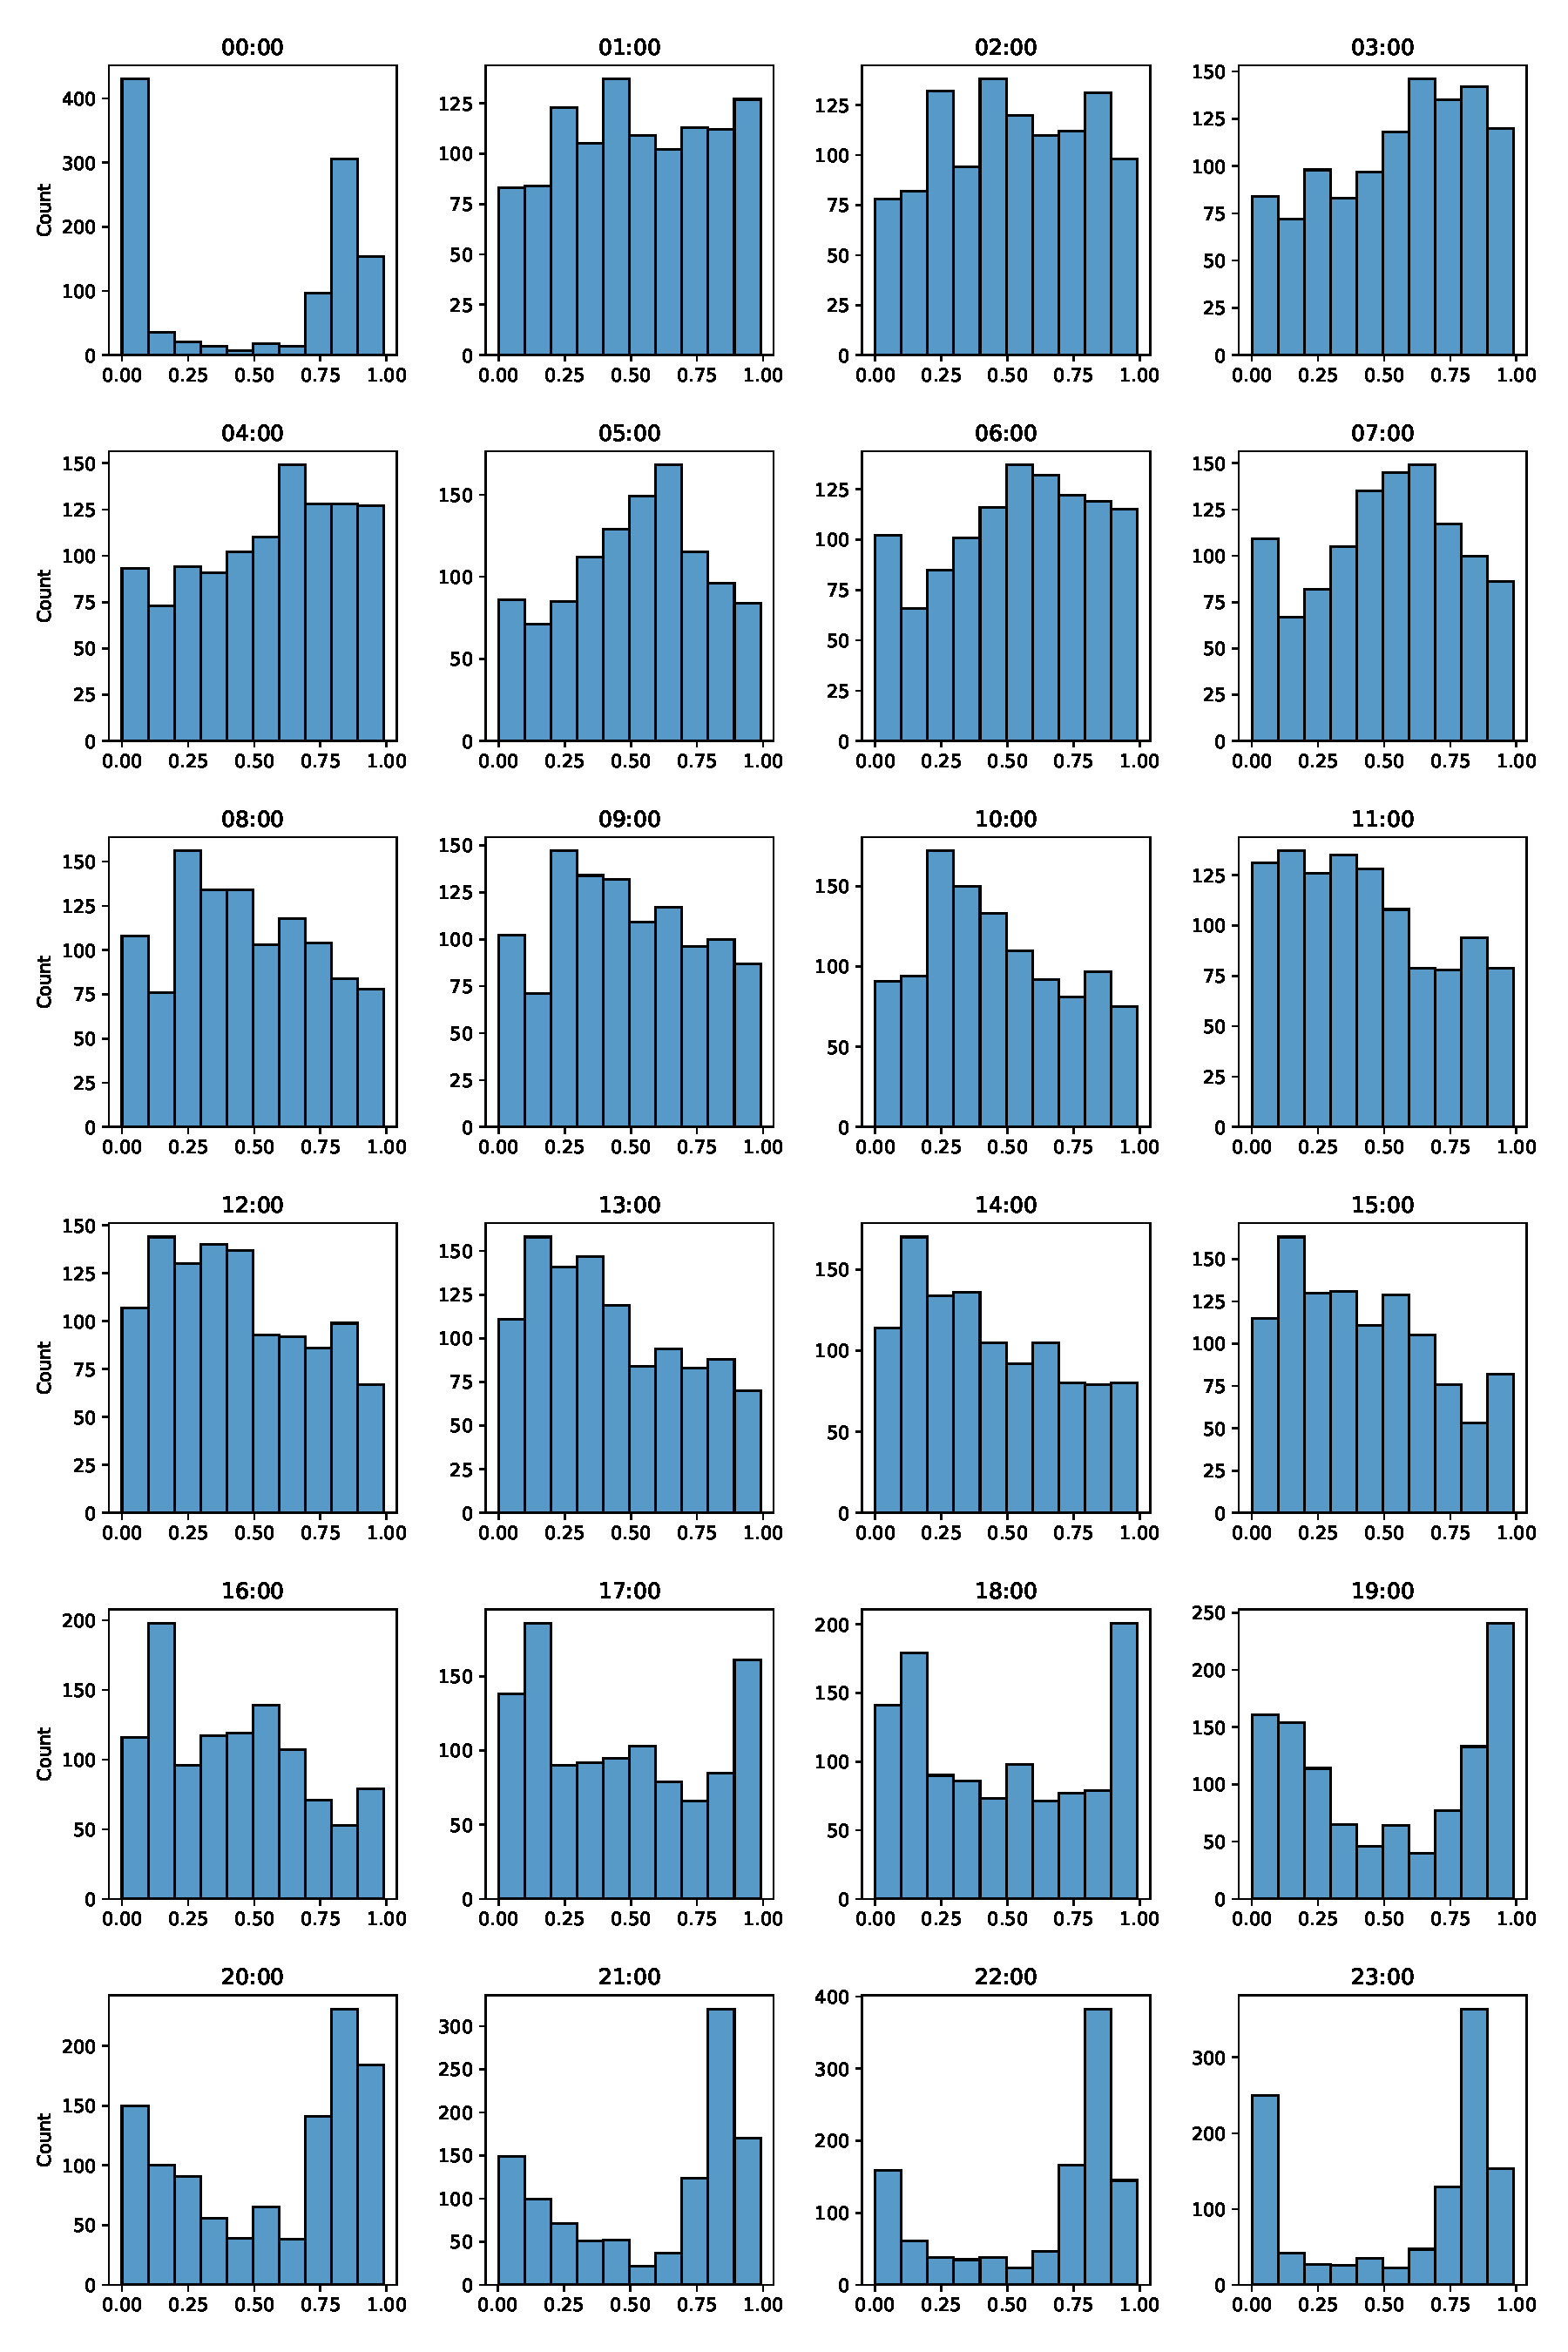
\includegraphics[width=\textwidth]{plots/pit/pit_by_hour_qrf.pdf}
    \caption[PIT histograms QRF]{PIT histograms of QRF. Since the model performs differently 
    in each hour, the PIT histogram is broken down into each hour.}%
    \label{fig:pit-qrf-by-hour}%
\end{figure}

\begin{figure}[h]%
    \centering
    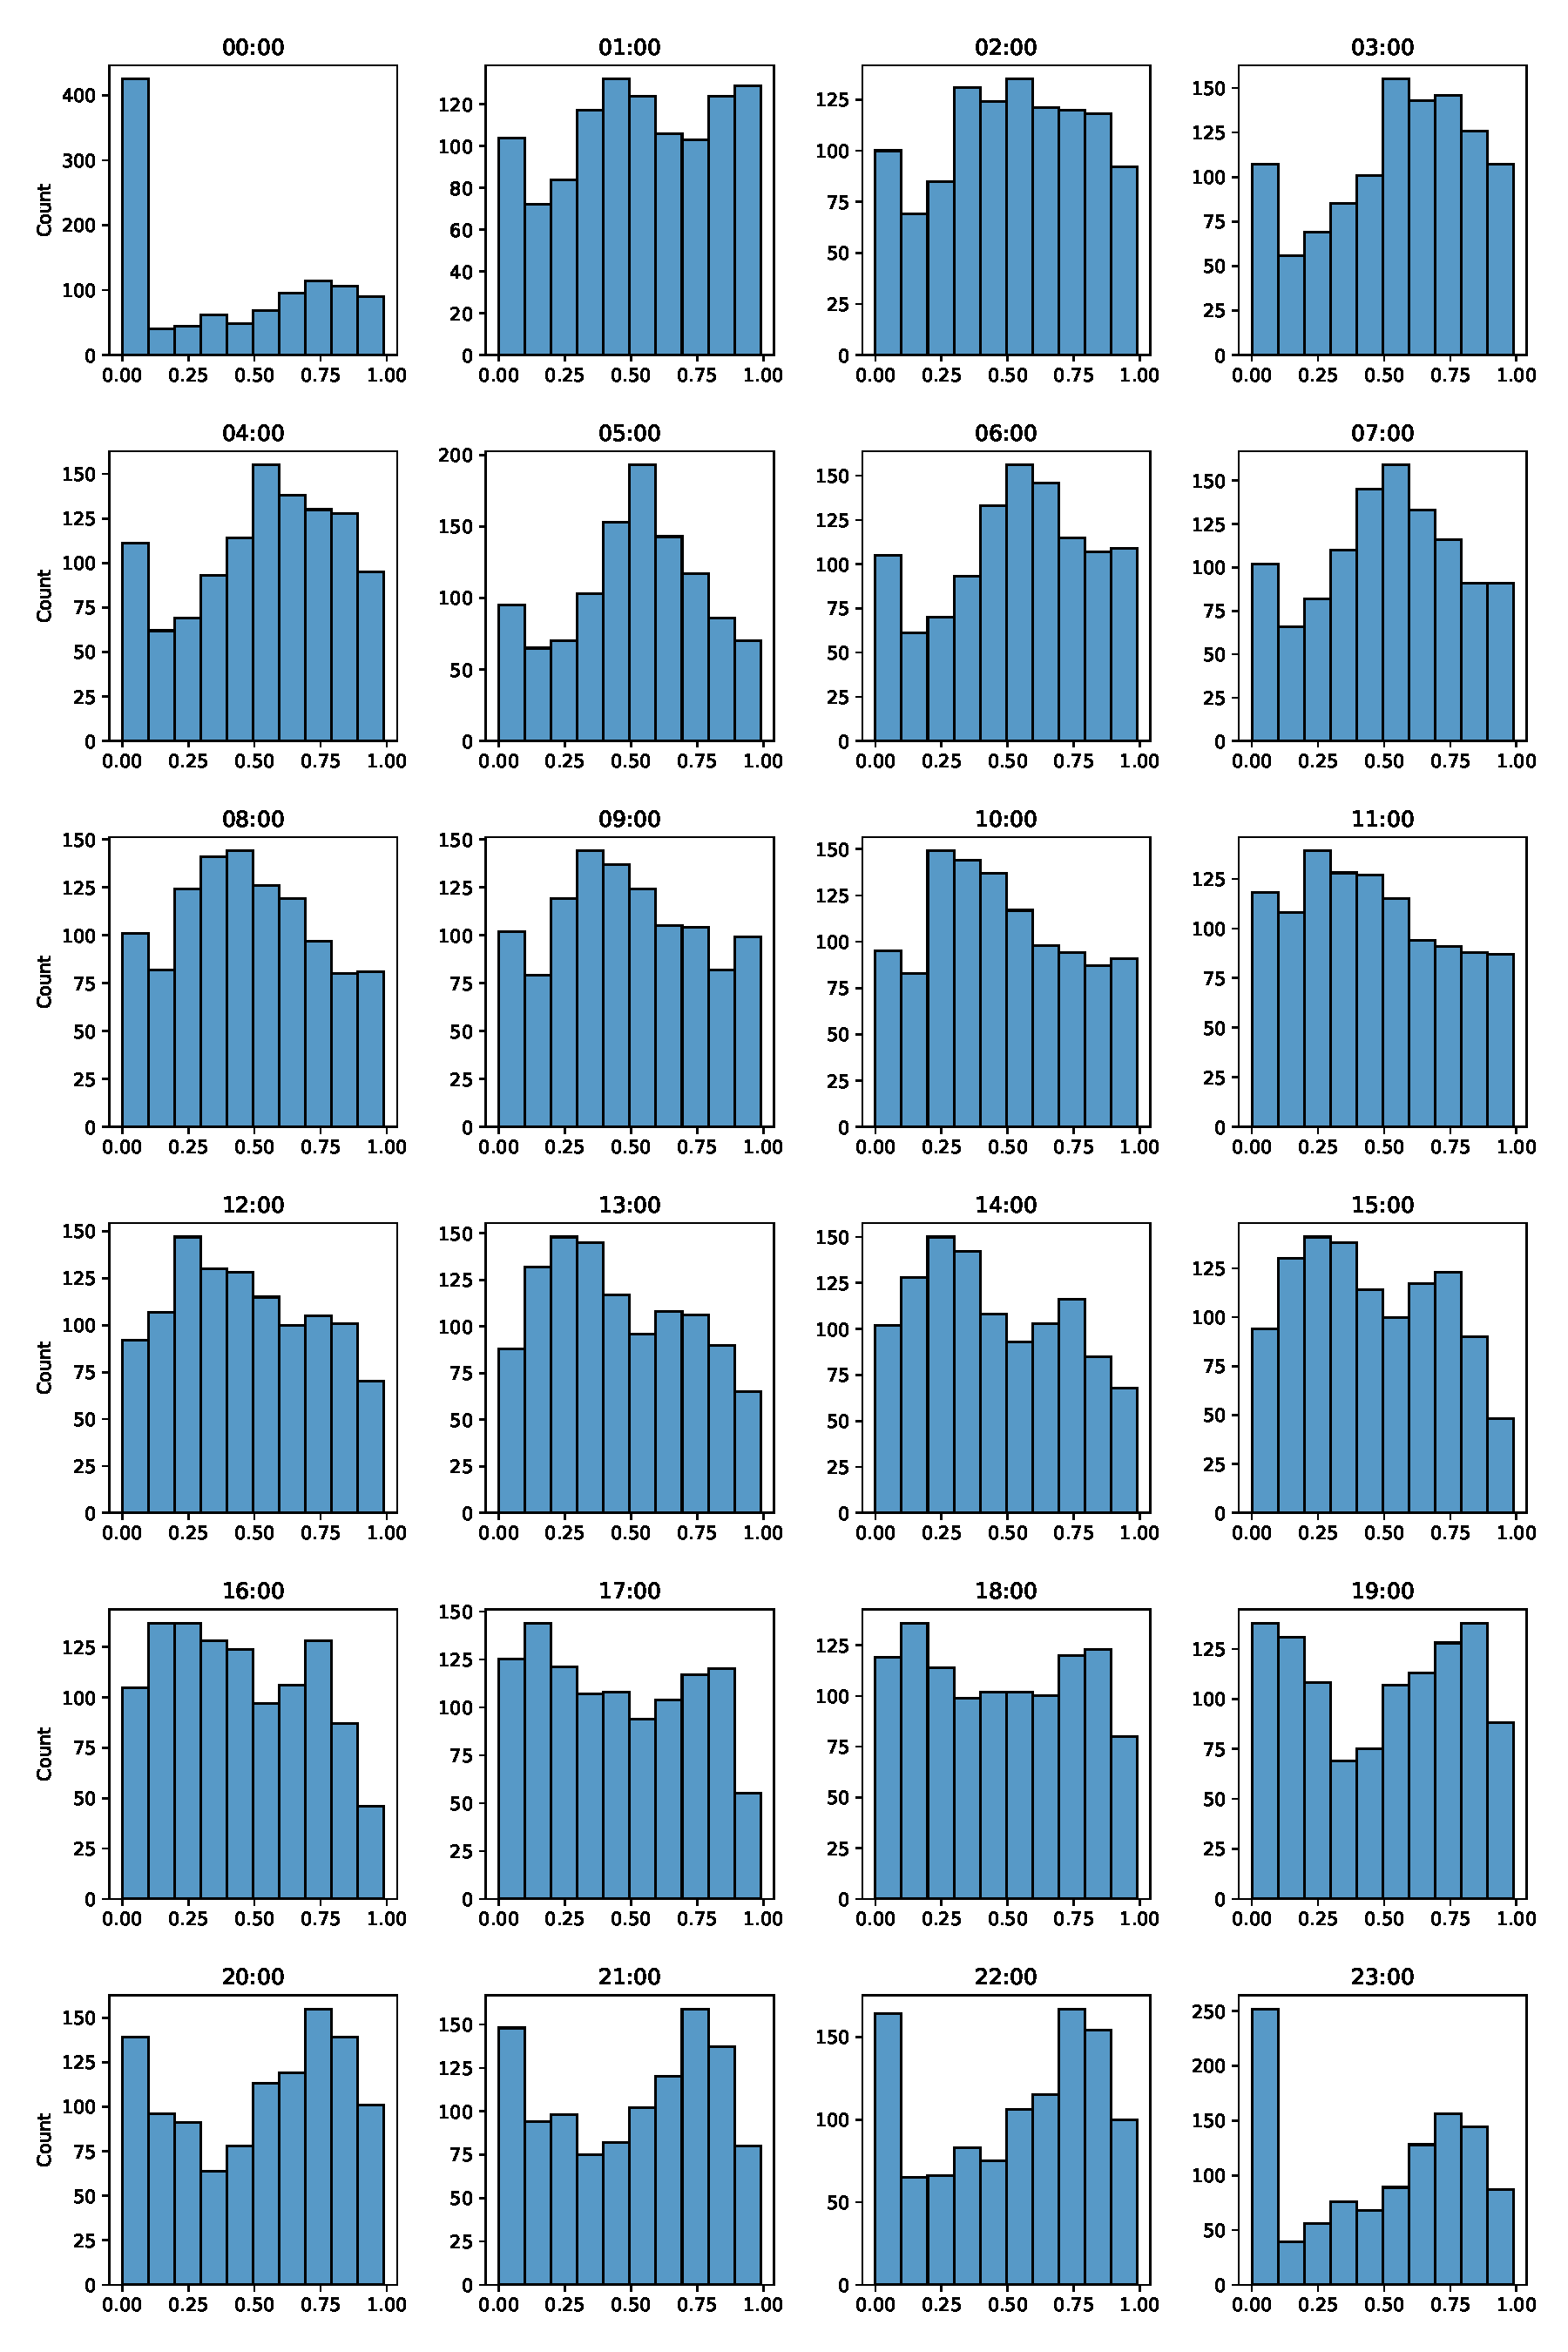
\includegraphics[width=\textwidth]{plots/pit/pit_by_hour_nnqf.pdf}
    \caption[PIT histograms NNQF]{PIT histograms of NNQF. Since the model performs differently 
    in each hour, the PIT histogram is broken down into each hour.}%
    \label{fig:pit-nnqf-by-hour}%
\end{figure}

\begin{figure}[h]%
    \centering
    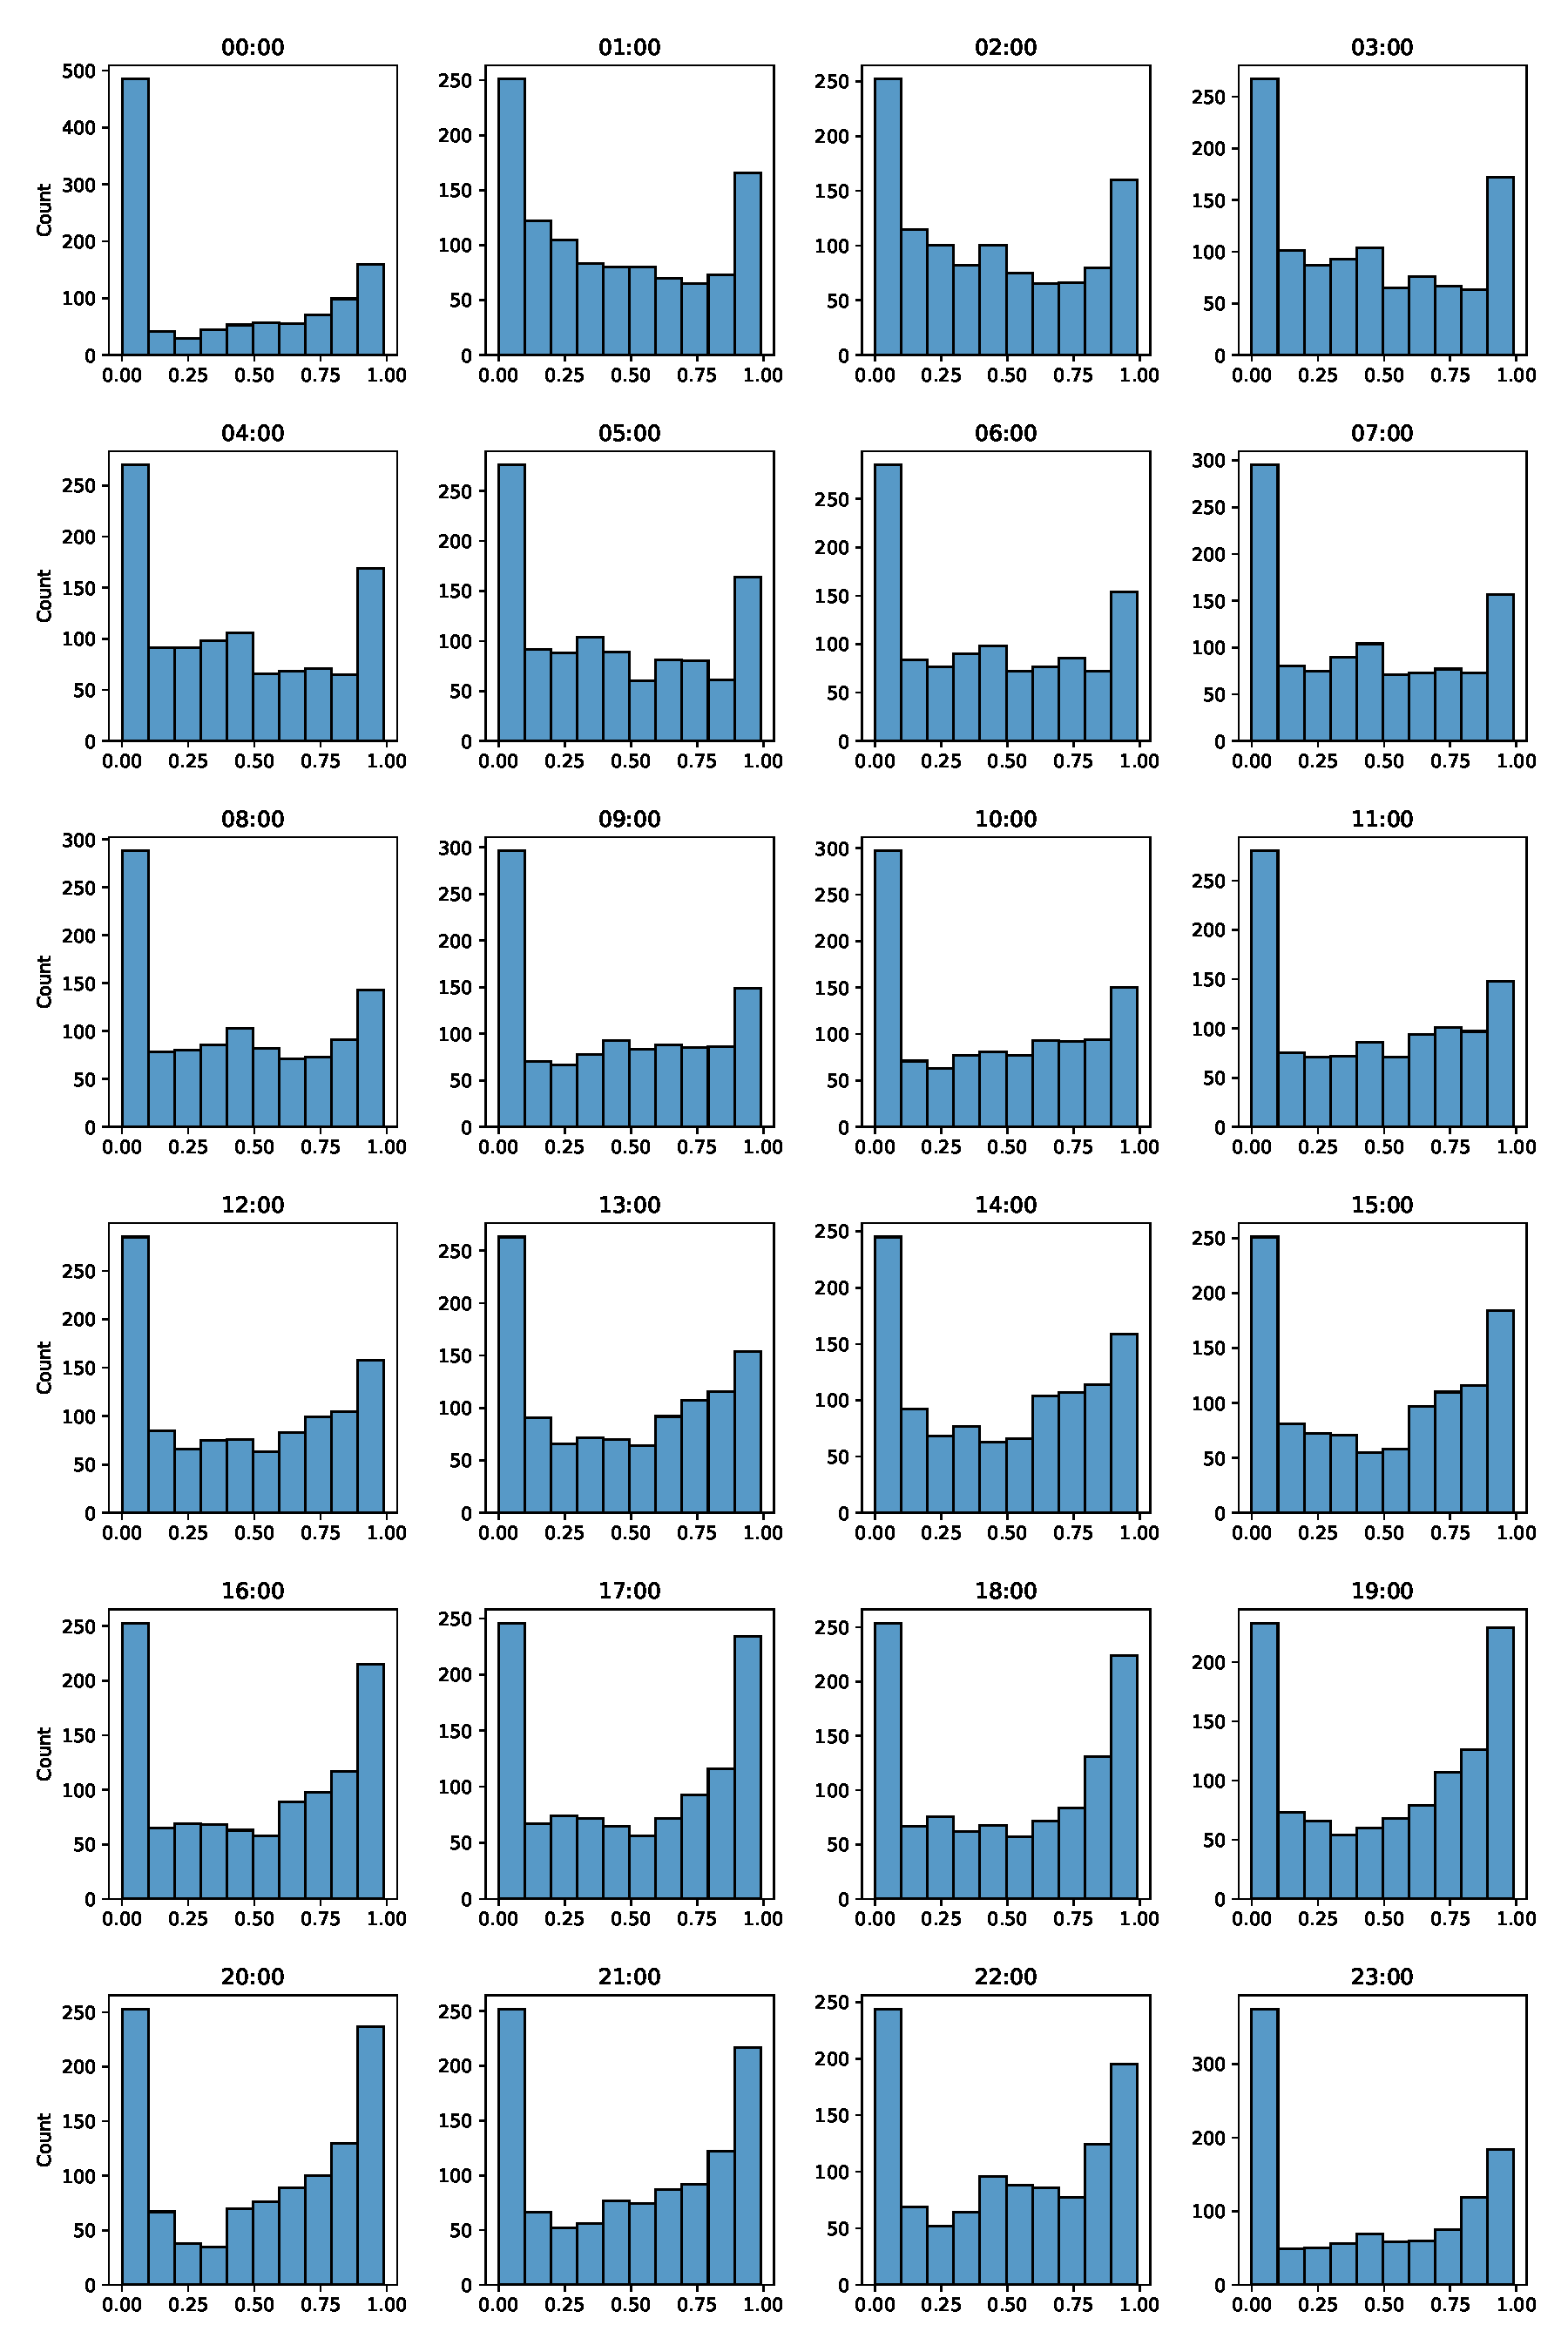
\includegraphics[width=\textwidth]{plots/pit/pit_by_hour_deepar.pdf}
    \caption[PIT histograms DeepAR]{PIT histograms of DeepAR. Since the model performs differently 
    in each hour, the PIT histogram is broken down into each hour.}%
    \label{fig:pit-deepar-by-hour}%
\end{figure}

\begin{figure}[h]%
    \centering
    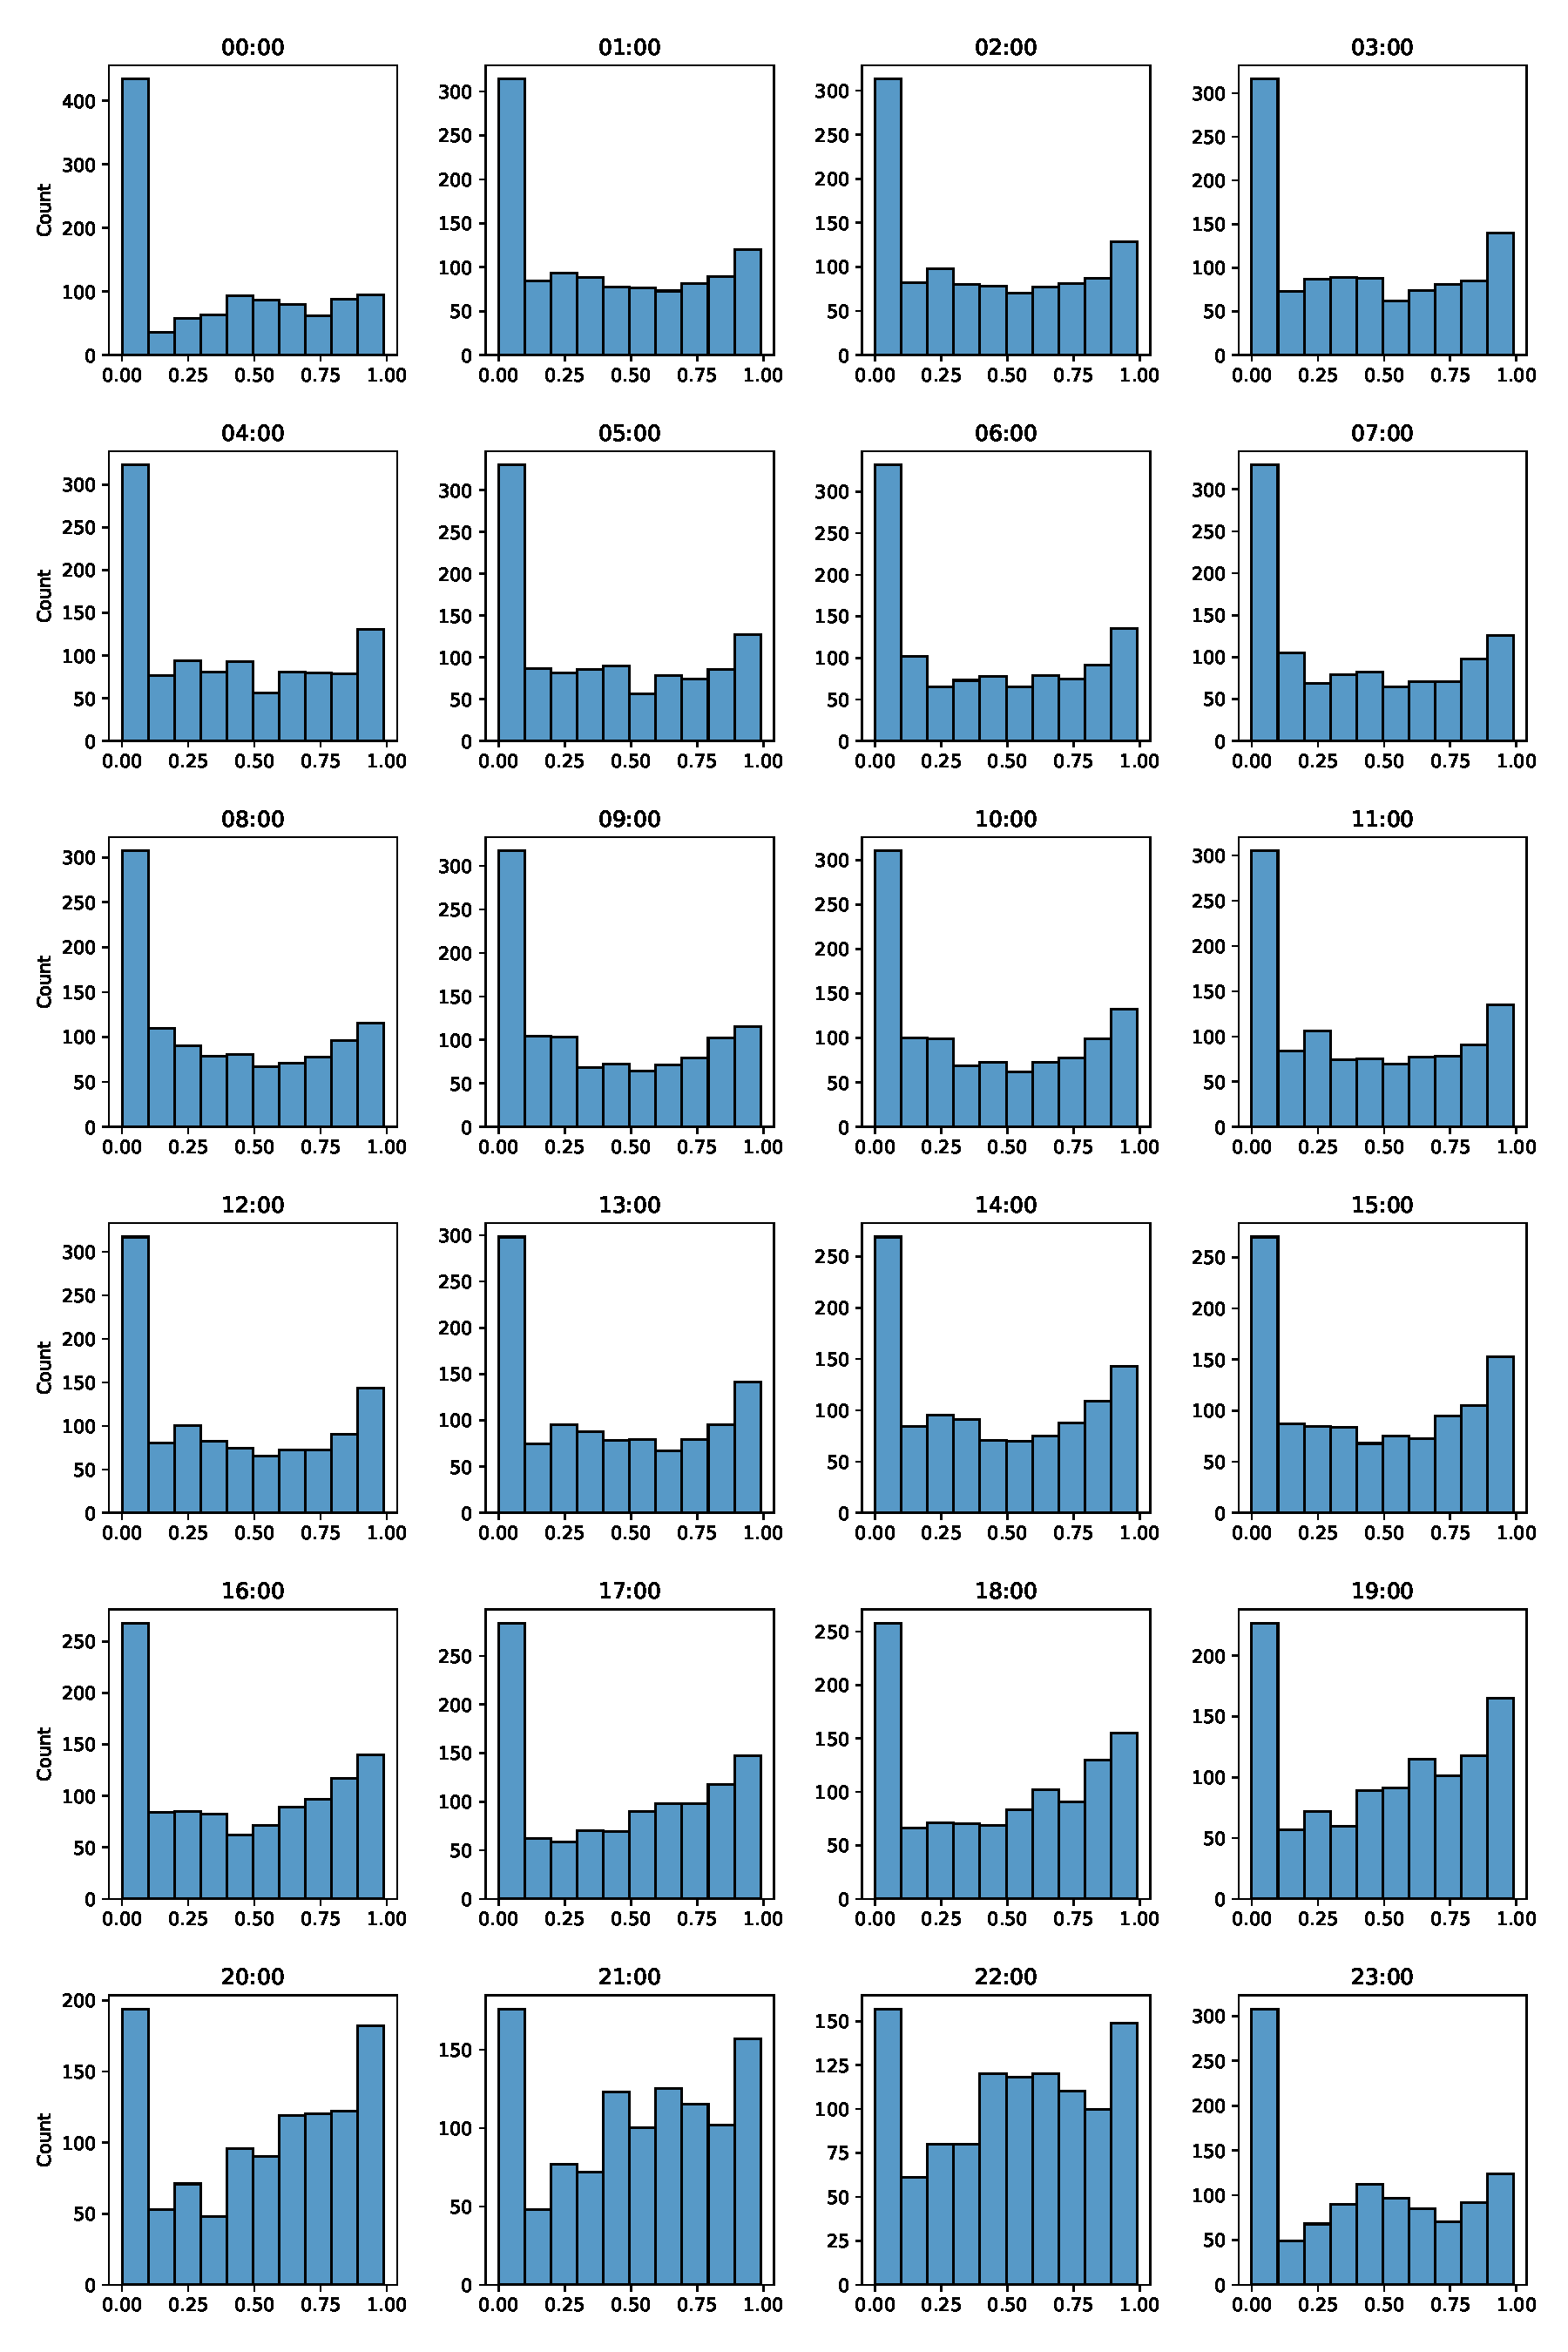
\includegraphics[width=\textwidth]{plots/pit/pit_by_hour_sqf-rnn.pdf}
    \caption[PIT histograms SQF-RNN]{PIT histograms of SQF-RNN. Since the model performs differently 
    in each hour, the PIT histogram is broken down into each hour.}%
    \label{fig:pit-sqf-rnn-by-hour}%
\end{figure}

\end{document}